\subsection{Computer Vision}
    \framepic{graphics/computervision/computer-vision}{
        \framefill
        \textcolor{white}{Computer Vision}
        \vskip 0.5cm
    }
    \begin{frame}{Computer Vision}
        \begin{block}{Classification Task}
            To determine to which of a set of \textbf{categories} a given object belongs to.
        \end{block}
        \begin{columns}[onlytextwidth]
            \column{0.3\textwidth}
            \centering
            \includegraphics[width=\textwidth]{graphics/computervision/classification-image.jpeg}
            \onslide <2-> {
                \column{0.4\textwidth}
                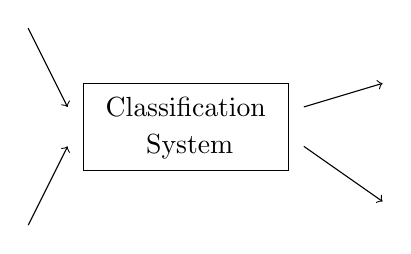
\begin{tikzpicture}
                    \node at (0,0) {Classification};
                    \node at (0.05,-0.5) {System};
                    \node[rectangle, draw, minimum width=2.6cm, minimum height=1.1cm, anchor=north west] at (-1.3,0.3) {};
                    \draw[->] (-2,1) -- (-1.5,0);
                    \draw[->] (-2,-1.5) -- (-1.5,-0.5);
                    \onslide <3-> {
                        \draw[->] (1.5,0) -- (2.5,0.3);
                        \draw[->] (1.5,-0.5) -- (2.5,-1.2);
                    }
                \end{tikzpicture}
            }
            \onslide <3-> {
                \column{0.2\textwidth}
                \vskip -0.5cm Output \vskip 0.5cm
                \begin{columns}[onlytextwidth]
                    \column{0.5\textwidth}
                        \begin{tabular}{|c|}
                            \hline
                            $0.03$\\\hline
                            \cellcolor{UniBlue}\textcolor{white}{$0.77$}\\\hline
                            $\vdots$\\\hline
                            $0.12$\\\hline
                        \end{tabular}
                    \column{0.5\textwidth}
                        \vskip -0.2cm
                        \begin{tabular}{c}
                            \\
                            \textcolor{UniBlue}{Child}\\
                            \\
                            \\
                        \end{tabular}
                \end{columns}
            }
        \end{columns}
    \end{frame}

    \begin{frame}{Computer Vision}
        \begin{block}{Object Localization Task}
            To find a given number (usually one) of items in a given context, predicting both their position and their class. \\
            \textbf{Remark.} Position is usually given as a bounding box.
        \end{block}
        \begin{columns}[onlytextwidth]
            \column{0.45\textwidth}
            \onslide <2-> {
                \includegraphics[width=\textwidth]{graphics/computervision/localization-input}
            }
            \column{0.45\textwidth}
            \onslide <3-> {
                \includegraphics[width=\textwidth]{graphics/computervision/localization-output}
            }
        \end{columns}
    \end{frame}

    \begin{frame}{Computer Vision}
        \onslide<1-> {
            \begin{block}{Object Detection Task}
                To \textbf{localize} any number of items in a given context, allowing either zero or any finite number of objects.
            \end{block}
        }
        \onslide<2-> {
            \begin{alertblock}{Remark.}
                The constraint on the number of object is \emph{a priori}. Indeed, a localization system will always look for a fixed number of objects, whereas a detection system is trained to be able to spot a variable number of objects in each input.
            \end{alertblock}
        }
    \end{frame}

    \begin{frame}{Computer Vision}
        \onslide <1-> {
            \begin{block}{Image Segmentation}
                Pixel-wide classification of the image. \textbf{Remark.} Image segmentation can be consider either the preemptive step to classification or the output of a classification system.
            \end{block}
        }
        \onslide <2-> {
            \vskip -0.5cm 
            \begin{exampleblock}{Example: Pixel-based image segmentation.}
                This family considers some distance defined over the image domain to segmentate it.
            \end{exampleblock}
        }
        \onslide <3-> {
            \vskip -0.5cm 
            \begin{exampleblock}{Example: Edge-based image segmentation.}
                This family uses an edge-detector algorithm, along with denoising and thresholding considerations, to solve the boundary detection problem.
            \end{exampleblock}
        }
    \end{frame}

    % \begin{frame}
    %     \frametitle{Pixel-based image segmentation}
    %     \framesubtitle{Whatershed}
    %     \begin{columns}[onlytextwidth]
    %         \column{0.5\textwidth}
    %         \includegraphics[width=\textwidth]{graphics/computervision/whatershed-plane}
    %         \column{0.5\textwidth}
    %         \includegraphics[width=\textwidth]{graphics/computervision/whatershed-surf}
    %     \end{columns}
    %     \only <1> {
    %         \begin{block}{Whatershed and immersion}
    %             The above pictures both show the same function defined over a 2D domain. Suppose to immerse the above right surface in some liquid, which gradually fill the two holes.
    %         \end{block}
    %     }
    %     \only <2> {
    %         \begin{block}{Whatershed and immersion}
    %             At some point the two volumes of liquid will meet, in particular they will flood at the same time over the green colored surface region.
    %         \end{block}
    %     }
    %     \only <3> {
    %         \begin{block}{Whatershed and immersion}
    %             This region is called whatershed and differentiates two areas of the image. Hence, an image can be segmentated considering its whatersheds.
    %         \end{block}
    %     }
    % \end{frame}

    % \begin{frame}
    %     \frametitle{Pixel-based image segmentation}
    %     \framesubtitle{Whatershed}
    %     % \includegraphics[width=\textwidth]{graphics/whatershed-plane}
    %     TODO insert example image\\
    %     % \includegraphics[width=\textwidth]{graphics/whatershed-surf}
    %     TODO insert example image
    % \end{frame}

    % \begin{frame}
    %     \frametitle{Pixel-based image segmentation}
    %     \framesubtitle{Whatershed}
    %     Let $\mathcal{D} \subset \mathbb{R}_+^2$ be a $2D$ domain, and $\mathcal{I} \colon \mathcal{D} \rightarrow \mathbb{R}_+$. Denote $\displaystyle h_m \triangleq \min_{\underline{x} \in \mathcal{D}}\mathcal{I}(\underline{x})$, $\displaystyle h_M \triangleq \max_{\underline{x} \in \mathcal{D}}\mathcal{I}(\underline{x})$, $T_h\left(\mathcal{I}\right) \triangleq \left\{\underline{p} \in \mathcal{D}, \mathcal{I}(\underline{p}) \leq h\right\}$.
    % \end{frame}

    % \begin{frame}
    %     \frametitle{Pixel-based image segmentation}
    %     \framesubtitle{Whatershed}
    %         \begin{itemize}
    %             \item Def, th, alg
    %             \item Example results
    %         \end{itemize}
    % \end{frame}

    \subsection{Alpha-shape}
    \begin{frame}{$\alpha$-Shape}
        \begin{columns}[onlytextwidth]
            \column{0.5\textwidth}
                \onslide <1-> {
                    \includegraphics[width=\textwidth]{graphics/computervision/detector-points}
                }
                \vskip -.7cm
                \onslide <4-> {
                    \includegraphics[width=\textwidth]{graphics/computervision/detector-convhull}
                }
            \column{0.5\textwidth}
                \onslide <2-> {
                    \includegraphics[width=\textwidth]{graphics/computervision/detector-a-shape}   
                }
                \vskip -.7cm
                \onslide <3-> {
                    \includegraphics[width=\textwidth]{graphics/computervision/detector-a-shape-better-radius}
                }
            
        \end{columns}
    \end{frame}

    \subsection{Optimization}
    \begin{frame}
        \frametitle{Optimization}
        \onslide <1-> {
            \begin{block}{Bayesian optimization}
                Bayesian optimization aims to solve an optimization problem $\max\limits_{x\in A}f\left(x\right)$ when:
                \begin{itemize}
                    \item $A \subset \mathbb{R}^d$ with $d$ not too large.
                    \item Easy to asses $A$ membership.
                    \item $f$ can be modeled using \emph{Gaussian process regression}.
                    \item $f$ is a \emph{black box}.
                \end{itemize}
            \end{block}
        }
        \onslide <2-> {
            \begin{exampleblock}{Loss function}
                \begin{equation}
                    J\left(\alpha\right) = \frac{2\lvert X \cap Y \rvert}{\lvert X \rvert + \lvert Y \rvert} = -f(x)
                \end{equation}
            \end{exampleblock}
        }
    \end{frame}
    
    \begin{frame}
        \frametitle{Optimization}
        \vskip -0.5cm
        \begin{block}{Bayesian optimization}
            Firstly a collection of points $x_1, \ldots, x_k \in \mathbb{R}^d$ is considered. Suppose $f$ can be modeled as:
            \begin{equation*}
                f\left(x_{1:n}\right) \sim \mathcal{N}\left(\mu\left(x_{1:n}\right), \Sigma\left(x_{1:n}, x_{1:n}\right)\right)
            \end{equation*}
            Then we can infere the probability distribution of $f\left(x_{n+1}\right)$:
            \begin{equation}
                f\left(x_{n+1}\right) \mid f\left(x_{1:n}\right) \sim \mathcal{N}\left(\mu_{n+1}, \Sigma_{n+1}\right)
            \end{equation}
            \begin{equation*}
                \mu_{n+1} = \Sigma\left(x_{n+1}, x_{1:n}\right)\Sigma\left(x_{1:n}, x_{1:n}\right)^{-1}\left(f\left(x_{1:n}\right) - \mu\left(x_{1:n}\right)\right) + \mu\left(x_{n}\right)
            \end{equation*}
            \begin{equation*}
                \Sigma_n = \Sigma\left(x_{n+1}, x_{n+1}\right) - \Sigma\left(x_{n+1}, x_{1:n}\right)\Sigma\left(x_{1:n}, x_{1:n}\right)^{-1}\Sigma\left(x_{1:n}, x_{n+1}\right)
            \end{equation*}
        \end{block}
    \end{frame}
    
    \begin{frame}
        \frametitle{Optimization}
        \begin{exampleblock}{Acquisition function}
            Therefore, it is possible to consider an \emph{acquisition function}, i.e. a function that given the previous $x_1, \ldots, x_n$ values determines the best choice of $x_{n+1}$:
            \begin{equation}
                a \colon \left[x_1 \ldots x_n\right] \rightarrow x_{n+1} \colon \mathcal{P}\left[f(x_{n+1}) = \max\limits_{x \in A} f\left(x\right)\right] \text{is max}
            \end{equation}
        \end{exampleblock}
    \end{frame}